Bei diesem Experiment spielt energiereiche Strahlung eine Rolle, die mit Materie
wechselwirkt. Es wird sowohl $\gamma$-Strahlung in einem Energiebereich von
$60\keV$ bis $1300\keV$, also auch $\beta^{-}$-Strahlung betrachtet. Beide
Strahlungsarten stammen von instabilen Kernen.

Wechselwirkung zwischen den emmitierten Photonen beziehungsweise Elektronen mit
Materie treten nur auf, wenn die Teilchen aufeinander treffen. Dies führt zu einer
Abnahme der Intensität der Strahlung.
Der Wirkungsquerschnitt $\sigma$ wird verwendet, da Materie zu einem großen Teil
aus Freiraum besteht. Hierbei gilt: je größer die Wahrscheinlichkeit ist, das
Teilchen miteinander Wechselwirken, desto größer ist der Wirkungsquerschnitt.

Ausschlaggebend für die Anzahl von Wechselwirkungen ist die Dicke $\su{D}$ des
verwendeten Absorbers. Für $\gamma$-Strahlung gilt ein exponentieller Abfall der
Intensität in Abhängigkeit der Dicke:
\begin{equation}
  N(D) = N_0 \cdot \exp^{-n\sigma D}.
  \label{eqn:steig}
\end{equation}
Hierbei ist $N_0$ die Ausgangsaktivität und $n$ die Anzahl der Teilchen im Absorber.
Der Absorptionskoeffizient $\mu$ wird durch $n\cdot\sigma$ definiert. Um die
Teilchenanzahl im Absorber zu berechnen wird die Formel
\begin{equation}
  n = \frac{z\su{N_L}}{\su{V_{mol}}} = \frac{z\su{N_L}\rho}{M}
\end{equation}
verwendet. Hierbei ist $\su{N_L}$ die Loschmidt'sche Zahl\cite{los} mit dem Wert
\begin{equation*}
  \su{N_L} = 2,687\,\cdot10^{25}\frac{1}{\mt^3}
\end{equation*}
Die Ordnungszahl wird durch $z$ beschrieben
und $M$ ist das Molekulargewicht.

\subsection{\texorpdfstring{Eigenschaften von $\gamma$}{(Eigenschaften von gamma)}-Strahlung}
Werden angeregte Atomkerne um ein oder mehrere Energieniveaus erniedrigt, wird
$\gamma$-Strahlung freigesetzt. Da es sich bei diesen Energieniveaus um diskrete
Zustände handelt, erhält man ein diskretes Linienspektrum für $\gamma$-Strahler.
$\gamma$-Strahlung breitet sich mit Lichtgeschwindigkeit aus, da sie aus Photonen
besteht. Zudem weist sie Eigenschaften auf, die für elektromagnetische Wellen
typisch sind.
Bei der Wechselwirkung von $\gamma$-Strahlung treten je nach Partner
unterschiedliche Effekte auf, wie in Abbildung \ref{fig:ww} gezeigt
\begin{figure}[H]
  \centering
  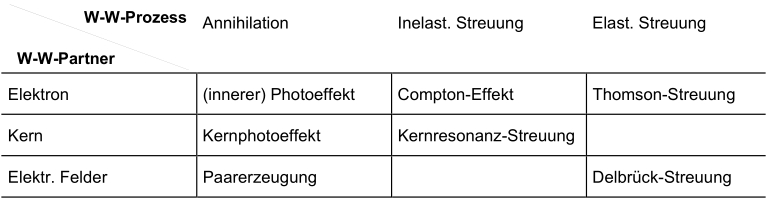
\includegraphics[width=0.6\textwidth]{bilder/wechselgamma.jpg}
  \caption{Mögliche Effekte von Wechselwirkung zwischen $\gamma$-Strahlung
  und Wechselwirkungspartner \cite{704}.}
  \label{fig:ww}
\end{figure}
Der Photo-Effekt, der Compton-Effekt und die Paarbildung treten mit am häufigsten
auf.
Beim Photo-Effekt wird ein Elektron aus der Absorberschale durch ein einfallendes
Photon gelöst. Das Photon gibt bei diesem Prozess seine gesamte Energie an das
Elektron ab und wird daraufhin vernichtet. Die Energieabgabe erfolgt jedoch nur,
wenn die Bindungsenergie $\su{E_B}$ überwunden wurde. Das hat zur Folge, dass
Photonen eine Grenzenergie besitzen müssen, damit es zum Photo-Effekt kommen kann.

\begin{wrapfigure}{r}{7cm}
  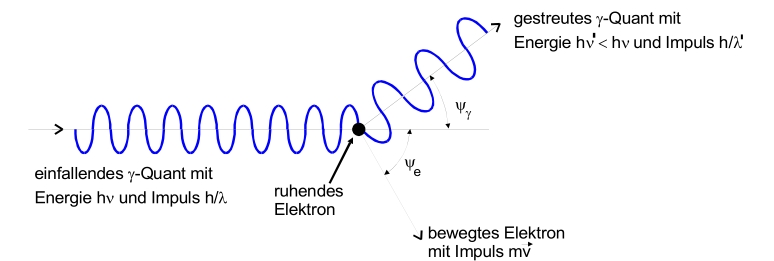
\includegraphics[width=7cm]{bilder/compton.jpg}
  \caption{Darstellung des Compton-Effekts \cite{704}.}
  \label{fig:com}
\end{wrapfigure}
Anders als beim Photo-Effekt, wird das Photon beim Compton-Effekt nicht vernichtet,
da beim stoßen mit dem Elektron nur ein Teil der Photonen-Energie abgegeben wird.
Bei diesem Prozess werden beide Teilchen wie in Abbildung \ref{fig:com} gezeigt,
von ihrer Bahn abgelenkt.
Für diesen Prozess wurde der Wirkungsquerschnitt $\sigma_\su{com}$ von Klein und
Nishina in Abhängigkeit von der Quantenenergie aufgestellt, sodass
\begin{equation}
  \sigma_\su{com}= 2\pi r^2_\su{e}\lf(\frac{1+\epsilon}{\epsilon^2}\lf[\frac{2(1+
  \epsilon)}{1+2\epsilon}-\frac{\ln(1+2\epsilon)}{\epsilon}\rt]+\frac{\ln(1+2\epsilon)}
  {2\epsilon}-\frac{1+3\epsilon}{(1+2\epsilon)^2}\rt)
  \label{eqn:sigma}
\end{equation}
gilt. Hierbei ist $r_\su{e}$ der Elektronenradius mit $r_\su{e}=2.818\,\cdot10^
{-15}\mt$ \cite{rad} und $\epsilon$ das Verhältnis von Quantenenergie und Ruheenergie
des Elektrons.
Beim Compton-Effekt ist der Wirkungsquerschnitt proportional zur Ordnungszahl $z$,
da dieser als Wechselwirkung mit freien Elektronen aufgefasst werden kann.
Der Absorptionskoeffizient $\mu_\su{com}$ berechnet sich dann mit
\begin{equation}
  \mu_\su{com}=n\sigma_\su{com}(\epsilon)=\frac{zN_\su{L}\rho}{M}\sigma_\su{com}
  (\epsilon).
  \label{eqn:mu}
\end{equation}

Bei der Paarbildung wird das Photon annihiliert, wenn die Energie des $\gamma$-Quants
mindestens doppelt so groß ist, wie die Ruhemasse eines Elektrons. Bei der
Annihilation entstehen ein Eletron und ein Positron.
Während der Photo-Effekt ausschließlich bei niederen Energien für die Bildung des
Absorptionskoeffizienten beteiligt ist, ist die Paarbildung bei hohen Energien
ausschlaggebend. Die Angleichung im mittleren Bereich erfolgt durch den
Compton-Effekt.
\subsection{Eigenschaften von \texorpdfstring{$\beta$}{beta}-Strahlung}
$\beta$-Strahlung entsteht bei dem Zerfall des Atomkerns und bestehen aus
Elektronen mit hoher Geschwindigkeit.
\begin{wrapfigure}{l}{7cm}
  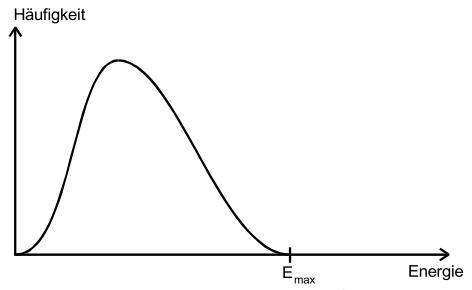
\includegraphics[width=7cm]{bilder/emissionbeta.jpg}
  \caption{Kontinuierliches Emissionsspektrum von $\beta^-$-Strahlung}
  \label{fig:emib}
\end{wrapfigure}
Während des Kernzerfalls, zerfällt ein Neutron zu einem Proton, einem Elektron
und einem Antineutrino $\bar\nu_\su{e}$.
\begin{equation*}
  n \rightarrow \su{p + \beta^- + \bar\nu_\su{e}}
\end{equation*}
Hierbei verteilt sich die Energie kontinuierlich auf das Antineutrino und das
Elektron. Abbildung \ref{fig:emib} zeigt das so entstehende kontinuierliche Spektrum.
Das Elektron kann eine Maximalenergie von $E_\su{max}$ erreichen, welche beim
gesamten Zerfallsprozess freigesetzt wird.
Wenn beim Durchlaufen des Absorbermaterials Streuungsprozesse auftreten, werden
häufig genug dieser Prozesse durchgeführt, sodass das Elektron nicht vollständig
Absorbiert wird oder austritt.
Bei der elastischen Streuung am Atomkern treten nur geringe Energieverluste auf.
Durch das Coulombfeld des Kerns werden die Elektronen jedoch teilweise sehr stark
abgelenkt. Das hat eine Intensitätsabnahme durch Auffächerung des Strahls zur Folge.
Weiter wird die Wechselwirkungs-Wahrscheinlichkeit durch das Verlängern der
Elektronenbahnen im Absorbermaterial stark verlängert.
Werden die $\beta$-Strahlen im Coulombfeld beschleunigt, besteht die Möglichkeit,
dass sie am Atomkern inelastisch gestreut werden. Dabei wird Energie in Form
von elektromagnetischer Strahlung abgegeben, die $\beta$-Teilchen bremst. Diese
Strahlung wird auch als Bremsstrahlung bezeichnet.

Für natürliche $\beta$-Strahler gilt ebenfalls ein exponentieller Abfall der
Intensität, bis die Schichtdicke nah an der maximalen Reichweite der Teilchen liegt.
Nach der maximalen Reichweite $\su{R_{max}}$ tritt nur noch Untergrundstrahlung auf.
Diese setzt sich aus Brems- und Hintergrundstrahlung zusammen. Logarithmiert man
beide Strahlungsintensitäten und stellt sie wie in Abbildung \ref{fig:reich}
\newpage
\begin{wrapfigure}{r}{7cm}
  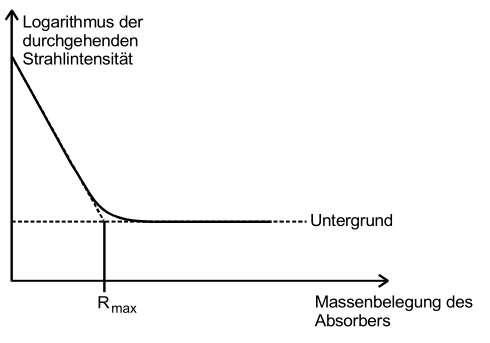
\includegraphics[width=7cm]{bilder/betaabsorp.jpg}
  \caption{Bestimmung der maximalen Reichweite von $\beta$-Strahlung.\cite{704}}
  \label{fig:reich}
\end{wrapfigure}
graphisch dar, kann auf die maximale Reichweite geschlossen werden. Die verwendete
Massenbelegung $R$ wird durch
\begin{equation}
  R=\rho D
\end{equation}
berechnet. Da hauptsächlich Teilchen mit der größten Energie die maximale Reichweite
bestimmen, lässt sich die maximale Energie $\su{E_max}$ mit Formel
\begin{equation}
  \su{E_{max}} = 1.92 \cdot\sqrt{\su{R_{max}}^2+0.22\,\cdot\su{R_{max}}}
  \label{eqn:emax}
\end{equation}
berechnen.
